\documentclass{beamer}
\usetheme{Madrid}

\usepackage{pifont}
\usepackage{enumitem, xcolor}
\usepackage{graphicx}
\usepackage{subcaption}

% default path to images and other assets
\graphicspath{{assets/}}

% disable wrapping
\tolerance=1
\emergencystretch=\maxdimen
\hyphenpenalty=10000
\hbadness=10000

% number figure caption
\setbeamertemplate{caption}[numbered]

% display bib label in references
\setbeamertemplate{bibliography item}{\insertbiblabel}
\setbeamertemplate{bibliography entry title}{}
\setbeamertemplate{bibliography entry location}{}
\setbeamertemplate{bibliography entry note}{}

% props and cons lists
\newlist{propslist}{itemize}{1}
\setlist[propslist]{label=\textcolor[HTML]{3C8031}{\ding{51}}}
\newlist{conslist}{itemize}{1}
\setlist[conslist]{label=\textcolor{red}{\ding{54}}}

% Metadata
% ------------------------
\title[Scientific metrics]{Comparison of different measures of scientific productivity and bibliography}

\author[O. Shkalikov \and M. Zannini \and Q.Qaribiyan]
{Oleh Shkalikov \and Matteo Zannini \and Qader Qaribiyan}

\institute[]{TU Dresden, Computer Science Faculty}

\date{December, 2022}

% ------------------------

\begin{document}

\frame{\titlepage}

\begin{frame}
    \frametitle{Agenda}
    \tableofcontents
\end{frame}

\section{Introduction}

\begin{frame}

    \frametitle{Scientific Productivity}

    Scientific productivity

   \hspace{1cm}

    how much output does a scientist produce within a certain time period

   \hspace{1cm}

   The major outputs from the research :

   \hspace{1cm}
    \begin{itemize}
      \item  Publications
      \item Patents
      \item  Product developments
    \end{itemize}
Among the publication forms, peer-reviewed journal articles are most frequently used as a productivity measure.
\end{frame}

\begin{frame}

    \frametitle{Bibliometric Incentive}

    \begin{figure}[h]
        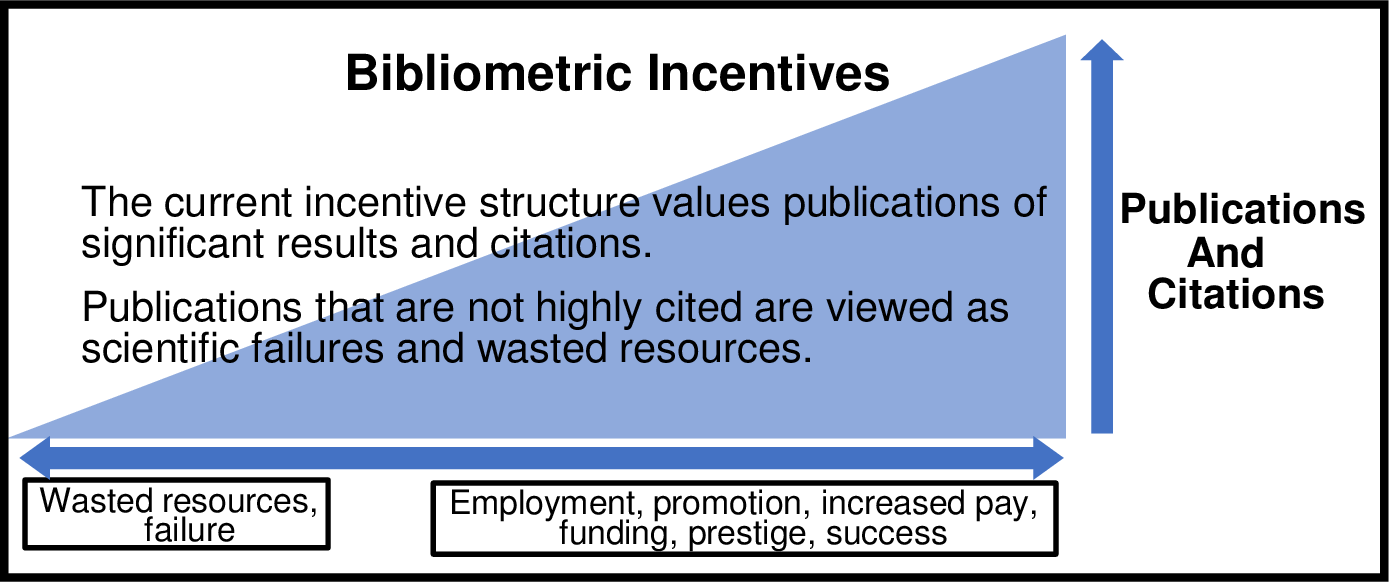
\includegraphics[height=0.5\textheight]{1.png}
        \caption{The current bibliometrics incentives model.}
    \end{figure}

\end{frame}

\section{Bibliometrics}

% Use section and subsection to add item to table of contents
\subsection{Impact factor}
\begin{frame}
    \frametitle{Impact factor}
    The Impact Factor is the average number of citations received by articles in a journal within a two-year window
    
    \begin{align*}
        IF(x) &= \frac{ Citations(x)}{ Publications(x - 2 ) +  Publications(x - 1) }\\
    \end{align*}

    For example, Nature had an impact factor of 49.962 in 2020:
    
    \begin{align*}
        IF(2020) &= \frac{ Citations(2020)}{ Publications(2018) +  Publications(2019) } &= 49.962\\
    \end{align*}

    Note that 2020 impact factors are reported in 2021; they cannot be calculated until all of 2020
    publications have been processed by the indexing agency.

\end{frame}
\begin{frame}
    \frametitle{Impact factor limitations}
    \begin{columns}[T]
        \begin{column}{.5\textwidth} \pause
            \centering Props
            \begin{propslist}
                \item it helps compare journals of the same field. It gives an idea of the journal’s relative importance and reputation. \pause
            \end{propslist}
        \end{column}
        \begin{column}{.5\textwidth}
            \centering Cons % example how to center one block
            \begin{conslist}
                \item The Impact Factor is an arithmetic mean and doesn’t adjust for the distribution of citations \pause
                \item Citations are only included if they appeared in a journal listed in the Citation Indexes \pause
                \item Impact Factors can show significant variation year-on-year.  \pause
                \item Not every journal has an Impact Factor.  \pause
            \end{conslist}
        \end{column}
    \end{columns}


\end{frame}
\begin{frame}
    \frametitle{Altmetric Attention Score}
    The Altmetric Attention Score tracks a wide range of online sources to capture the conversations happening around academic research.
    

\end{frame}


\section{Researcher's metrics}

\begin{frame}
    \frametitle{Blocks and columns and simple animation}

    \begin{block}{Sample ordinary block}
        You can use \textit{columns} environment to
        split a slide into 2 or more parts.
    \end{block}

    \begin{alertblock}{Props and cons lists}
        Use \textit{propslist} and \textit{conslist} enveroments
        to show props and cons as a list respectively.
    \end{alertblock}

    \begin{columns}[T]
        \begin{column}{.5\textwidth} \pause
            \centering Props
            \begin{propslist}
                \item First benefit \pause
                \item Second benefit \pause
            \end{propslist}
        \end{column}
        \begin{column}{.5\textwidth}
            \centering Cons % example how to center one block
            \begin{conslist}
                \item First disadvantage \pause
                \item Second disadvantage \pause
                \item Third disadvantage \pause
            \end{conslist}
        \end{column}
    \end{columns}

    \begin{exampleblock}{Sample example block}
        Example: For example you can implement props and cons
        with use of columns.
    \end{exampleblock}

\end{frame}

\begin{frame}
    \frametitle{Sample citations}

    \begin{block}{Citation in \LaTeX\ with Bibtex}
        To cite something just add your
        bibitem in \textit{references.bib} file and
        use \textit{cite} command with corresponding name.
        Everything else will happen \textbf{automatically}!
    \end{block}

    I claim something very important and have to
    cite this paper \cite{goodfellow2014generative},
    this article \cite{unet},
    book \cite{pix2pixHD}
    and preprint \cite{pix2pix}.

    \begin{alertblock}{Where to find citation bibtex item}
        Please use citation \textit{BibTeX} item
        from Google Scholar
    \end{alertblock}

\end{frame}

\begin{frame}
    \frametitle{Inserting images}

    \begin{figure}[h]
        
\includegraphics[height=0.3\textheight]{TU_Dresden_Logo_blau_HKS41.jpg}
        \caption{Big picture}
    \end{figure}

    If you want 2 side image, use \textit{subfigures}
    \begin{figure}[h]
        \begin{subfigure}{0.49\textwidth}
            \centering
            
\includegraphics[width=0.7\textwidth]{TU_Dresden_Logo_blau_HKS41.jpg}
            \caption{White}
        \end{subfigure}
        \begin{subfigure}{0.49\textwidth}
            \centering
            
\includegraphics[width=0.7\textwidth]{TU_Dresden_Logo_invers.jpg}
            \caption{Blue}
        \end{subfigure}
        \caption{Main caption}
    \end{figure}
\end{frame}

\begin{frame}[allowframebreaks]
    \frametitle{References}

    \bibliographystyle{apalike}
    \bibliography{references.bib}

\end{frame}

\end{document}